% !TeX encoding = UTF-8
% maindoc

\documentclass[a4paper,12pt,oneside,german,toc=bibliography]{scrbook} 

\usepackage[ngerman]{babel}
\usepackage[utf8]{inputenc}
\usepackage{amsmath,amsthm,amssymb,amsfonts,amscd,amsbsy,amsxtra,amsthm}

\usepackage[alphabetic,nobysame,bibtex-style]{amsrefs}
\makeatletter
\renewcommand\PrintNames@a[4]{%
    \PrintSeries{\name}
    {#1}
    {}{ und \set@othername}
    {;}{ \set@othername}
    {}{ und \set@othername}
    {#2}{#4}{#3}%
}
\makeatother


\usepackage{dsfont}
\usepackage{enumerate}
\usepackage{graphicx}
\usepackage{subfig}
\usepackage{upgreek,textcomp}
\usepackage{cleveref}
\usepackage[Algorithmus]{algorithm}
\usepackage{algpseudocode}
\usepackage[autostyle=true,german=quotes]{csquotes}
\usepackage{ziffer}
\usepackage{booktabs}
\usepackage{courier}

\makeatletter
\newcommand{\specialcell}[1]{\ifmeasuring@#1\else\omit$\displaystyle#1$\ignorespaces\fi}
\makeatother

\usepackage[numbered,autolinebreaks,bw]{mcode}   %framed

\theoremstyle{definition}
\newtheorem{defn}{Definition}[section]
\newtheorem{bem}[defn]{Bemerkung}

\theoremstyle{plain}
\newtheorem{satz}[defn]{Satz}
\newtheorem{lem}[defn]{Lemma}
\newtheorem{prop}[defn]{Proposition}
\newtheorem{kor}[defn]{Korollar}

\numberwithin{equation}{section}

\DeclareMathOperator{\cond}{cond}
\DeclareMathOperator{\spn}{span}
\DeclareMathOperator{\diag}{diag}
\DeclareMathOperator{\eZahl}{e}
\DeclareMathOperator{\diff}{d}
\DeclareMathOperator{\imag}{i}

\newcommand{\ehoch}[1]{{\eZahl}^{#1}}



\newcommand{\R}{\mathds{R}}
\newcommand{\C}{\mathds{C}}
\newcommand{\N}{\mathds{N}}
\newcommand{\Q}{\mathds{Q}}
\newcommand{\la}{\lambda}
\newcommand{\calV}{\mathcal{V}}
\newcommand{\calF}{\mathcal{F}}
\newcommand{\calW}{\mathcal{W}}
\newcommand{\calP}{\mathcal{P}}
\newcommand{\calO}{\mathcal{O}}
\newcommand{\mPhi}{\mathit{\Phi}}
\newcommand{\eqItem}{\item~\vspace{-2\normalbaselineskip}}
\newcommand{\imaginary}{\mathrm{i}}
\newcommand{\LskalProd}{(\,\cdot\,,\,\cdot\,)_w}

\let\vphi=\phi
\renewcommand{\phi}{\varphi}

\newcommand{\transp}[1]{#1^\mathrm{T}}

\begin{document}

%!TEX root = /Users/mbantle/Dropbox/BantleM/Thesis/diplomarbeit.tex

\begin{titlepage}
	\begin{figure}[h]
		
\includegraphics[width=\textwidth]{images/unilogoA4}
	\end{figure}
	\vspace{1cm}
\begin{center}
{\large \bfseries Fakultät für Mathematik und Wirtschaftswissenschaften \\
\vspace{0.3cm}
\bfseries Institut für Numerische Mathematik \\
}
\vspace{2cm}
{\Large
Projekt CSE\\}

\vspace{2cm}
{\LARGE\bfseries
Radarsignalverarbeitung mit Grafikprozessoren\\
}
\end{center}

%
\vspace{3.5cm}
%
\begin{center}
%\vspace{0.2cm}
%{\bfseries\mbox{Anton Hügel}} \\
%\vspace{0.2cm}
%Zwischenstand vom \mbox{\today} \\

vorgelegt von \\
\vspace{0.2cm}
{\bfseries\mbox{Anton Hügel, Jonas Schwer, Lukas Tatzel, Michael Thoma}} \\
\vspace{0.2cm}
am \mbox{\today} \\

\vspace*{1.2cm}
{\bfseries Betreuung} \\
\mbox{}\\
\mbox{Prof. Dr. Stefan A. Funken, Dr. Markus Bantle} \\
\end{center}
\vfill
\end{titlepage}


\tableofcontents





%==========================================================================%
% Kapitel 1 - Theorie
%==========================================================================%

\chapter{Theorie}

% Überblick Kapitel und Quellen
In diesem Kapitel soll die Funktionsweise eines Radar-Systems (\textbf{ra}dio \textbf{d}etection \textbf{a}nd \textbf{r}anging) und dessen Signalverarbeitungsalgorithmen sowie einige mathematische Grundlagen kurz erläutert werden, wie sie in ausführlicher Form auch in \cites{Richards,RSH,Ludloff} nachzulesen sind. Zudem wird eine grundlegende Einführung in die Programmierschnittstelle OpenCL gegeben, mit welcher eine Programmierung für Grafikprozessoren umgesetzt werden kann.

\section{Funktionsweise eines Radars} 

% Zusammenfassung
Dieses Unterkapitel behandelt die Funktionsweise eines Radars. Falls nicht anders angegeben, stammen die hier zusammengetragenen Informationen aus \cite[Kapitel 1\&{}2]{Richards} und \cite[Kapitel 1]{Ludloff}.

% Hautaufgabe Radar und weitere Fähigkeiten
Die Hauptaufgabe eines Radars besteht darin, Objekte mittels Radiowellen zu detektieren und deren Position zu bestimmen. Dazu werden elektromagnetische Wellen über die Antenne des Radars emittiert. Diese werden an Objekten, die sich im Sichtfeld des Radars befinden, reflektiert und gelangen als \glqq  Echo\grqq ~wieder zum Radar zurück. Elektromagnetische Wellen bewegen sich in Luft (in guter Näherung) mit Lichtgeschwindigkeit, also mit knapp $ 300000 ~\text{km/s} $ fort. Die Zeit zwischen dem Aussenden und dem Empfangen der Radiowelle wird als \glqq Laufzeit\grqq ~bezeichnet. Anhand der Laufzeit, lässt sich über eine einfache Formel der Abstand zwischen dem Radar und einem reflektierenden Objekt berechnen. Neben der Entfernungsmessung sind moderne Radarsysteme dazu in der Lage, die Geschwindigkeit von detektierten Objekten zu messen (Doppler-Filterung), den Typ der Ziele zu bestimmen (Klassifikation) und deren Position nachzuverfolgen (Tracking).

% Radartypen, Überleitung zum Unterkapitel
Es gibt eine Vielzahl von verschiedenen Radar-Typen, die sich in ihrer Funktionsweise beispielsweise hinsichtlich der Sendefrequenz, Sendeleistung  oder Bauart unterscheiden. Dementsprechend existiert heute eine große Anzahl von Anwendungsmöglichkeiten, sowohl im zivilen als auch im militärischen Bereich. Im Zuge dieses Projekts wird ausschließlich ein sogenanntes \glqq Puls-Doppler-Radar\grqq ~betrachtet. 

%Puls-Doppler-Radar

\subsection{Puls-Doppler-Radar}

Beim Puls-Doppler-Radar werden durch die Antenne des Radars kurze Sendepulse in dieselbe Richtung emittiert. Auf jeden Sendepuls folgt eine gewisse Empfangszeit, in der die Antenne auf Empfang geschaltet wird. Ein Vorteil des Puls-Doppler-Radars besteht also in der Möglichkeit, eine einzige Antenne sowohl für das Senden als auch das Empfangen verwenden zu können. Vergleicht man einen Sendepuls mit dessen Echo, so stellt man bei bewegten Objekten einen Unterschied im Frequenzverlauf fest. Dieses Phänomen wird als \glqq Dopplereffekt\grqq ~bezeichnet. Durch den Vergleich von mehreren Echos verschiedener Sendepulse lassen sich Rückschlüsse auf die Geschwindigkeit (genauer die Radialgeschwindigkeit bezogen auf das Radar) von detektierten Objekten ziehen. Durch die obigen beiden Charakteristika kommt die Bezeichnung \glqq Puls-Doppler-Radar\grqq ~zustande. 

Die Zeitdauer, die für das Aussenden eines Pulses benötigt wird, heißt Pulsbreite und wird mit \( \tau \) bezeichnet (vgl. Abbildung \ref{fig:PRI}). Zusammen mit der Empfangszeit ergibt sich eine Zeitspanne, die PRI (Pulse Repetition Interval) genannt wird. Deren Kehrwert liefert die PRF (Pulse Repetition Frequency): $ 1/\text{PRI} = \text{PRF} $. Eine Folge mehrerer Einzelpulse, die in dieselbe Richtung abgegeben und gemeinsam verarbeitet werden, heißt \glqq Burst\grqq . Die Dauer eines Burst wird mit CPI (Coherent Processing Interval) bezeichnet. 
%
\begin{figure}[h] 
  \centering
     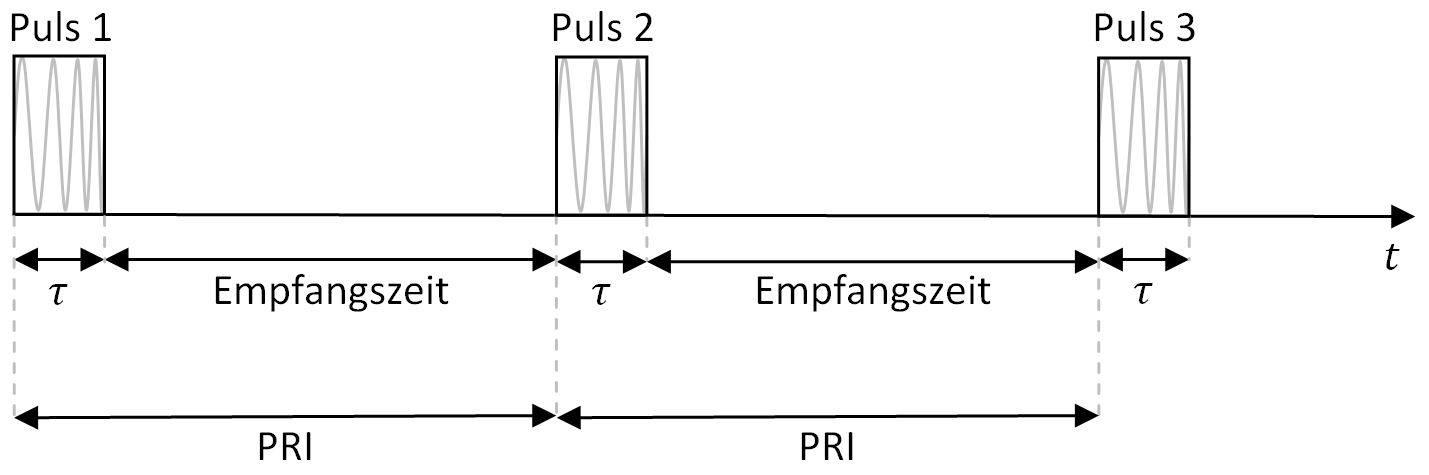
\includegraphics[scale=0.4]{images/Pulse_Radar_PRI_Zoom240.PNG}
  \caption{Schematische Darstellung von mehreren PRIs im Zeitbereich}
  \label{fig:PRI}
\end{figure} 
%




% Aufbau
\subsection{Aufbau eines Radar}

Die folgende schematische Darstellung des Aufbaus eines Puls-Doppler-Radars (vgl. Abbildung \ref{fig:Aufbau}) ist stark vereinfacht und auf das Projekt angepasst. Eine ausführlichere Darstellung der Komponenten eines Radars ist beispielsweise in \cite[Abschnitt 1.4]{Ludloff} oder \cite[Abschnitt 1.3]{Richards} zu finden. 

\begin{figure}[h] 
  \centering
  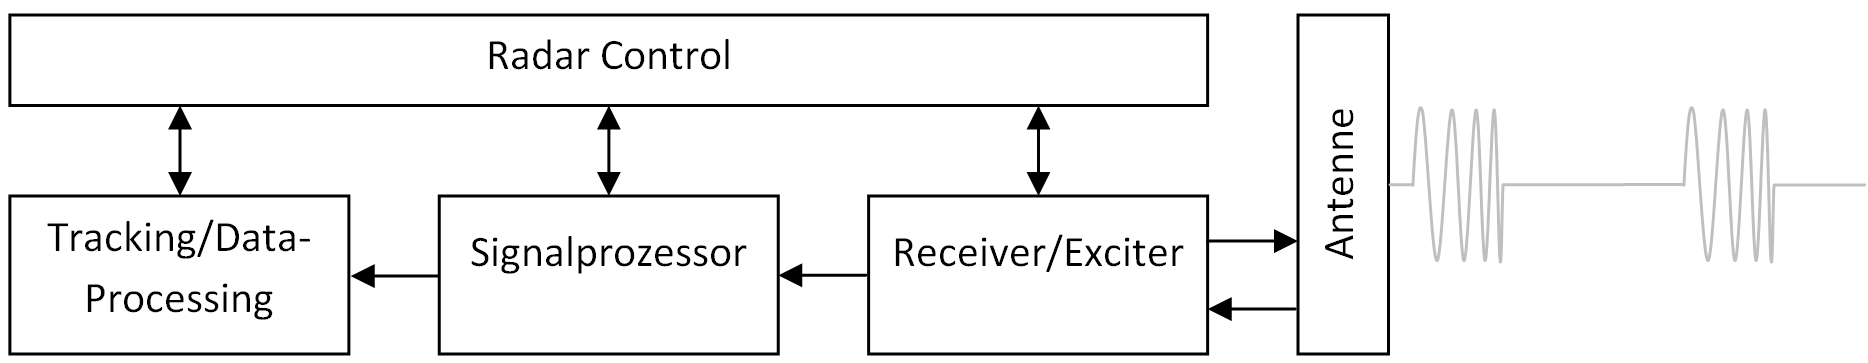
\includegraphics[scale=0.4]{images/Radar_Aufbau_Zoom240.PNG}
  \caption{Schematische Darstellung des Aufbaus eines Radars}
  \label{fig:Aufbau}
\end{figure}

Die Antenne sendet und empfängt elektromagnetische Signale. Diese beiden Phasen (Senden und Empfangen) laufen zyklisch, aber zeitlich getrennt voneinander ab, sodass beim Puls-Doppler-Radar eine Antenne ausreicht. Für das Aussenden der Signale wird der Exciter benötigt. Dieser erzeugt das Sendesignal, verstärkt es und mischt es vom sogenannten \glqq Basisband\grqq ~auf das \glqq Hochfrequenzband\grqq ~hoch (mehr dazu im folgenden Unterkapitel \ref{subsec:Signale}. Ist die Antenne auf Empfang geschaltet, so wird der Receiver aktiv. Dieser verstärkt und filtert  die empfangenen Signale und mischt sie auf das Basisband herunter (auch hierzu ist Genaueres in Kapitel \ref{subsec:Signale} zu finden. Der Receiver übernimmt des Weiteren die Aufgabe der Digitalisierung der bis dato analogen Daten. Die digitalisierten Daten werden im Signalprozessor weiterverarbeitet und analysiert. Ziel der Signalverarbeitung ist die Detektion von Zielen, sowie die Berechnung der Geschwindigkeiten, mit denen sich die Ziele fortbewegen. Beim Tracking/Data Processing werden die Detektionen weiterverarbeitet. Der gesamte Prozess wird durch die Radar Control gesteuert und koordiniert.

%Signale

\subsection{Sende- und Empfangssignale}
\label{subsec:Signale}

Dieses Unterkapitel behandelt die theoretischen Grundlagen zum Thema Sende- und Empfangssignale. Ziel ist es, einen realistischen Datensatz zu erzeugen, der dem Signalprozessor zur Weiterverarbeitung zur Verfügung gestellt werden kann. Wir wollen also ein konkretes Simulationsszenario vorgeben können und daraus einen Datensatz (in Form einer Matrix \(M_0)\) generieren, der den realen Gegebenheiten möglichst nahe kommt. Zu einem solchen Simulationsszenario gehören beispielsweise die Anzahl der Ziele im Sichtfeld des Radars (mit deren Radialgeschwindigkeit und Entfernung zum Radar), wie auch einige Parameter, die die Form des Sendepulses bestimmen.

Wir gehen in dieser Projektarbeit (nach Aufgabenstellung) von linear-fre\-quenz\-mo\-du\-lier\-ten Pulsen aus, das heißt, über die Pulsbreite $ \tau $ verändert sich die Sendefrequenz linear. Exemplarisch soll an dieser Stelle der erste Sendepuls des Burst, sowie dessen Echo für ein sich bewegendes Objekt im Sichtfeld des Radars vorgestellt werden. Ein linear-fre\-quenz\-mo\-du\-lier\-ter Puls hat die Form
% 
\begin{equation}
  s(t) := \exp\left( i \, \pi \, B \, (t - \tau/2)^{2}/{\tau} \right) 
        = \exp\left( i \, \Phi(t) \right), \quad t \in [0, \tau] 
\end{equation}
%
mit der Bandbreite \(B\) und der Pulslänge \(\tau\). Der Frequenzverlauf des Pulses ist demnach gegeben durch
%
\begin{equation}
  F(t) = \frac{1}{2\pi}\frac{\diff \Phi(t)}{\diff t} = \frac{B}{\tau}(t-\tau/2), \quad t \in [0, \tau] \text{.}
\end{equation}
% 
% !!! OPTIONAL !!!
%
%Wählt man beispielsweise $ B = 10^6~\text{Hz} $ und $ \tau = 30 \cdot %10^{-6}~\text{s} $, so ergibt sich der in Abbildung \ref{fig:Sendepuls} %dargestellte Sendepuls und Frequenzverlauf. 
%
%\begin{figure}[H] 
%  \centering
%     \includegraphics[scale=0.8]{images/%Sendepuls_und_Frequenzverlauf.png}
%  \caption{Linear-frequenzmodulierter Puls}
%  \label{fig:Sendepuls}
%\end{figure} 
%
% !!! OPTIONAL !!!
%
Grundsätzlich sind bei den Sende- und Empfangssignalen das \glqq Basisband\grqq ~und das \glqq Hochfrequenzband \grqq ~zu unterscheiden. Wie in Abbildung \ref{fig:Sendepuls} zu sehen ist, wird das Basisband durch die mittlere Frequenz Null charakterisiert. Tatsächlich sendet die Antenne elektromagnetische Wellen aber in einem höheren Frequenzbereich - dem Hochfrequenzband. Dafür wird der Frequenzverlauf des obigen Pulses um eine Frequenz $F_{c}$ (c für \glqq carrier\grqq) angehoben, die als \glqq Sendefrequenz\grqq ~oder \glqq Trägerfrequenz\grqq ~bezeichnet wird. Für den hochfrequenten Sendepuls $\overline{s}$ mit der mittleren Frequenz $F_{c}$ gilt also:
%
\begin{eqnarray}
& \overline{s}(t) &= s(t)\cdot  \exp\left( i \, 2 \pi \, F_{c} \, (t - \tau/2) \right) \\
& &= \exp\left( i \, \Phi(t) + i \, 2 \pi \, F_{c} \, (t - \tau/2) \right) 
\end{eqnarray}
%
für $ t \in [0, \tau] $. Dementsprechend gilt für den Frequenzverlauf
%
\begin{eqnarray}
& \overline{F}(t) &= \frac{B}{\tau}(t-\tau/2) + F_{c} \\
& &= F(t) + F_{c}
\end{eqnarray}
%
für $ t \in [0, \tau] $ . Die Simulation des Exciters ist an dieser Stelle abgeschlossen. Wir widmen uns nun dem Receiver und betrachten dementsprechend die Empfangssignale. Die Form und Position des Echosignals im Zeitbereich hängt im Wesentlichen von zwei Faktoren ab: Dem Abstand zwischen Radar und Ziel und der radialen Geschwindigkeit des Ziels. Um das Empfangssignal zu konstruieren, betrachten wir den Abstand zwischen Radar und Ziel als Funktion $ R(t) $. Wird vom Radar ein Sendepuls $ \overline{s}(t) $ ausgesendet, so lässt sich das Echo $ \overline{r}(t) $ beschreiben durch eine verzögerte Kopie des Sendepulses. Wir erhalten 
%
\begin{eqnarray}
& \overline{r}(t) = c_{mag} \cdot \overline{s}(t - \frac{2 R(t)}{c}) \text{,}
\label{eq:echo}
\end{eqnarray}
%
wobei $ c $ der Lichtgeschwindigkeit entspricht. Der Parameter $ c_{mag} $ dient dazu, die Stärke des reflektierten Signals berücksichtigen zu können (mag für \glqq magnitude\grqq). Dieser hängt beispielsweise von der Größe des Ziels ab. Obige Formel (\ref{eq:echo}) führt nach \cite[Seite 95]{Richards} zu einer korrekten Beschreibung des zeitabhängigen Dopper-Shifts. Geht man von einer Anfangsentfernung $ R_0 = R(t=0) $ und einer konstanten Radialgeschwindigkeit $ v_{r} $ des Ziels aus, dann gilt $ R(t) = R_0 - v_r\cdot t $. Eine positive Radialgeschwindigkeit entspricht dabei einem Ziel, das sich dem Radar nähert. Um das Basisband-Echosignal zu erhalten, verschieben wir den Frequenzverlauf des reflektierten Signals $ \overline{r}(t) $ um $ F_c $ nach unten, also
%
\begin{eqnarray}
& r(t) = \overline{r}(t)\cdot \exp\left(- i \, 2 \pi \, F_{c} \, (t - \tau/2) \right) \text{.}
\end{eqnarray}
%
Dieses Signal $ r(t) $ wird anschließend mit der Sampling-Frequenz  $ S $ abgetastet und in der entsprechenden Zeile der Matrix $ M_0 $ abgelegt. Die i-te Zeile $ (i = 1,...,M) $ der Matrix $ M_0 $ repräsentiert dabei den mit der Rate $ S $ abgetasteten/gesampelten Zeitbereich $ [\tau + (i-1)\cdot \text{PRI}, \enskip i\cdot \text{PRI}] $. Bei den Zeilen von $ M_0 $ spricht man auch von \glqq Slow Time Samples\grqq , während man die Spalten der Matrix als \glqq Fast Time Samples\grqq ~bezeichnet. Nach der Überlagerung der gesampelten Signale (jedes Ziel erzeugt ein Echo), wird noch weißes (d.h. normal verteiltes) Rauschen hinzugefügt. Mit der Matlab-Funktion \texttt{generate\_{}cpi\_{}return\_{}matrix.m} wird die Generierung der Matrix $ M_0 $ realisiert. Sie ist in \cref{chap:Quellcode} zu finden.

Zusammenfassend stellt die folgende Abbildung \ref{fig:ZusFas} schematisch den oben beschriebenen Ablauf von der Generierung des Sendepulses bis zum Abtasten des Basisband-Echosignals dar. 
%
\begin{figure}[H] 
  \centering
     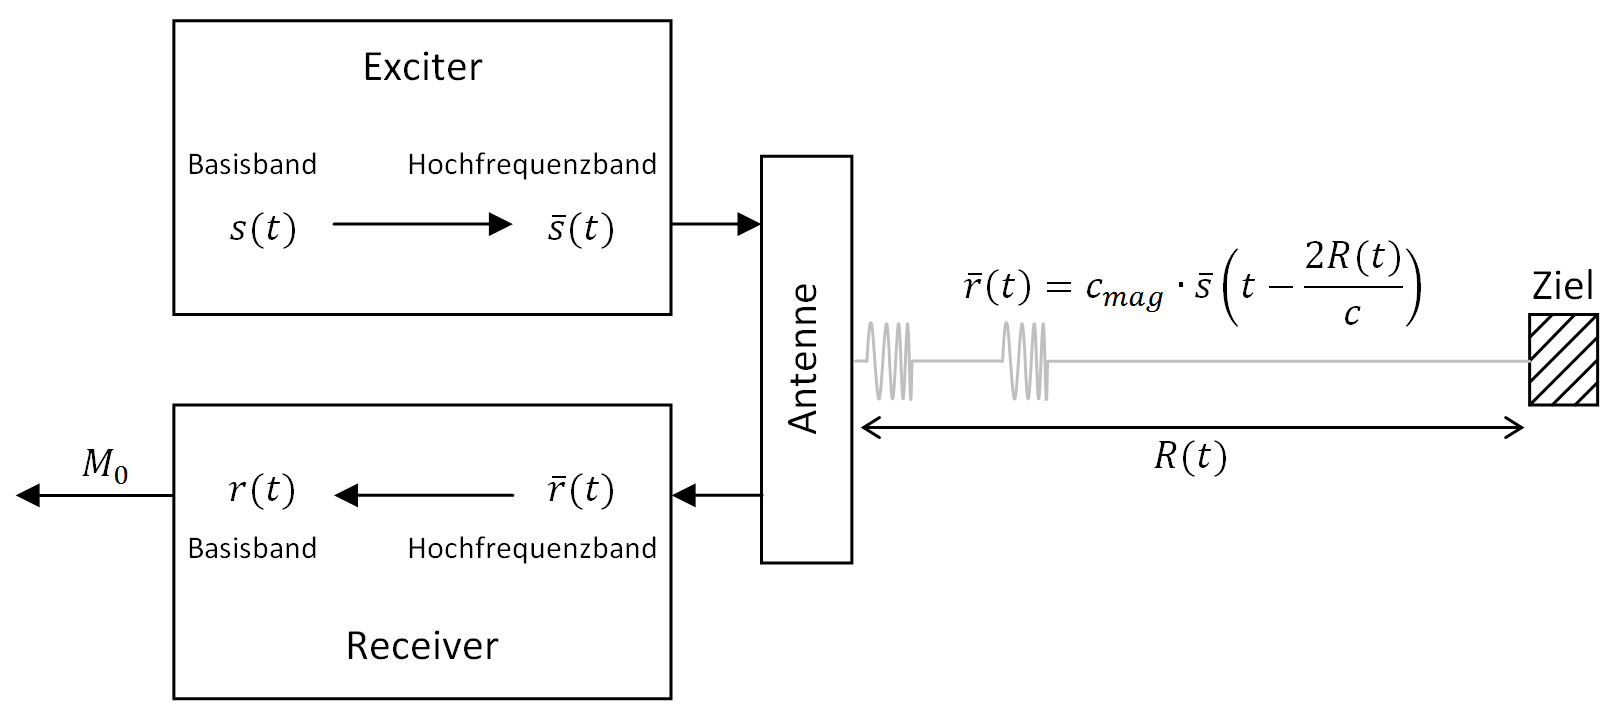
\includegraphics[scale=0.4]{images/Signals_Exciter_Receiver_Zoom240.PNG}
  \caption{Schematische Darstellung des Ablaufs}
  \label{fig:ZusFas}
\end{figure} 
%


%--------------------------------------------------------------------------%

\section{Radarsignalverarbeitung}

%Pulskompression

\subsection{Pulskompression}
Zunächst wird eine Pulskompression durchgeführt. Dies bewirkt, dass sich im Rauschen verborgene Echos in ihrer Amplitude verstärken und ihre Domäne sich verkleinert. Dadurch kann ein Echo sicher und scharf lokalisiert werden. Zunutze macht man sich hierbei das Prinzip des Optimalfilters (Matched Filter, \cite{RSH}*{20.2}), welcher im Empfangssignal nach einem Echo des Sendesignals sucht und dieses dann verstärkt. Dies geschieht, indem das Empfangene Signal mit dem Sendesignal gefaltet wird.
\begin{defn}
Sei $s:~[0,\tau] \to \C$ das Sendesignal und $r:~[\tau,\text{PRI}]\to\C$ das Empfangssignal. Die Pulskompression bzw. der Optimalfilter für diese Anwendung ist gegeben durch
\begin{displaymath}
G(r,s)(t) = a \int_{\Omega(t)} r(x)s^*(x-t)dx, \quad t\in [0,\text{PRI}],~\Omega(t)\subset\C,~a\in\R,
\end{displaymath}
wobei $\Omega(t)$ stets so gewählt wird, dass der Definitionsbereich von $s$ ausgeschlöpft wird.
Die Pulskompression entspricht also der Faltung des Empfangssignal mit dem zeitinvertierten und komplex konjugierten Sendesignal.
\end{defn}

Im jetzt betrachteten disrekten Fall, ist $r\in\C^n$ eine Zeile der Daten-Matrix $M_0$ und $s\in\C^p$ ein Vektor, der eine Abtastung des Sendesignals mit gleicher Rate beinhaltet. Der pulskomprimierte Datenvektor $y\in\C^{n+p}$ ergibt sich dann durch


\begin{displaymath}
y_k = a \sum_{j = \alpha}^{\beta} r_j s^*_{k-j+1}
\end{displaymath}
wobei
\begin{displaymath}
k=1,\ldots,n+p,\quad\alpha=\max\{0,k+1-n\},\quad\beta= \min\{k,m\}.
\end{displaymath}
%Dopplerfilterung

\subsection{Dopplerfilterung}
%Betrags-Bildung

\subsection{Betrags-Bildung}
%CFAR

\subsection{CFAR}


%--------------------------------------------------------------------------%

\section{Fouriertransformation}
Um ein genaueres Verständnis der Fouriertransformation (FT) zu geben, welche im letzten Abschnitt zur Gewinnung des Spektrums eines empfagenen Zeitsignal verwendet wurde, soll diese hier eingeführt und deren wichtigste Aussagen zusammengefasst werden. Zunächst wird die FT in ihrer allgemeinen, kontinuierlichen Form definiert, daraufhin wird sie für diskrete Signale untersucht und schließlich der Algorithmus der schnellen Fouriertransformation (FFT - Fast Fourier Transform) beschrieben. In Form der FFT kommt die Fouriertransformation in der in \cref{chap:Projekt} vorgestellten Implementierung zum Einsatz.

%KFT

\subsection{Kontinuierliche FT}

\begin{defn}[\cite{BurgHaf}*{Definition 8.3}]
    Sei $f: \R\to\R$ stückweise stetig und absolut integrierbar. Gilt für $\hat{f}: \R\to\R$ die Zuordnung
    \begin{displaymath}
        \hat{f}(s) = \frac{1}{2\pi} \int_{-\infty}^{\infty}  f(t) \ehoch{-{\imag}st} {\diff}t, \quad s\in\R ,
    \end{displaymath}
    so nennt man $\hat{f}$ die \emph{Fouriertransformierte von f}. Man schreibt für $\hat{f}$ auch $\calF f$. Der Operator $\calF$ heißt dann \emph{Fouriertransformation}.

\end{defn}

\begin{satz}[\cite{BurgHaf}*{Satz 8.1}]
    Ist $\hat{f}$ die Fourier-Transformierte von $f$, so gilt
    \begin{displaymath}
        f(t) = \int_{-\infty}^{\infty}  \hat{f}(s) \ehoch{{\imag}ts} {\diff}s, \quad t\in\R.
    \end{displaymath}
\end{satz}
\begin{proof}
    Siehe Quelle.
\end{proof}

\begin{satz}[\cite{BurgHaf}*{Satz 8.5}]
    Seien $f_1,f_2$ stetige, beschränkte und absolut integrierbare Funktionen in $\R$. Für deren Faltung $f_1 * f_2$ gilt:
    \begin{displaymath}
      \calF(f_1 * f_2) = \calF f_1 ~ \calF f_2.
    \end{displaymath}
\end{satz}
\begin{proof}
    Siehe Quelle.
\end{proof}


%DFT

\subsection{Diskrete Fouriertransformation}

In der Signalverarbeitung kann die Fouriertransformation als eine Abbildung aufgefasst werden, welche ein im Zeitbereich gegebenes, periodisches Signal in den Frequenzbereich überführt. Für eine sinuidale Schwingung erhält man mittels der Fouriertransformation die darin ethaltenen Frequenzen und deren Gewichtung. \\
Nun sind in der digitalen Signalverarbeitung jedoch nie zeitkontinuierliche Signale gegeben, sondern immer nur ein Daten-Vektor mit deren diskreter Abtastung. Dies motitivert, die Fouriertransformation auch für $N$-elementige Vektoren zu definieren, welche wir dann Diskrete Fouriertransformation (Descrete Fourier Transform, DFT) nennen.

\begin{defn}[\cite{BurgHaf}*{Definition 8.7}]

Die Abbildung $\calF_N: \C^N\to\C^N$, die einem Daten-Vektor $f=\transp{(f_0,\ldots,f_{N-1})} \in\C^N$ durch

\begin{displaymath}
\hat{c}_k = \frac{1}{N} \sum_{j=0}^{N-1} f_j \ehoch{-\imag 2 \pi k j/N} , k=0,\ldots, N-1
\end{displaymath}
den Vektor $\hat{c} = \transp{(\hat{c}_0,\ldots,\hat{c}_{N-1})} \in\C^N$ zuordnet, heißt \emph{diskrete Fouriertransformation mit $N$ Stützstellen}, DFT($N$).
\end{defn}

\begin{satz}[\cite{BurgHaf}*{Satz 8.9} und (8.84)-(8.87)]
Aussagen der Fouriertransformation lassen sich auf die diskrete Fouriertransformation übertragen.\newline
Sei $\hat{c} = \calF_N f$ zu einem Daten-Vektor $f=\transp{(f_0,\ldots,f_{N-1})} \in\C^N$.
\begin{enumerate}[(i)]
\item Für die \emph{inverse diskrete Fouriertransformation}  $\calF_N^{-1}: \C^N\to\C^N$ gilt:
    \begin{displaymath}
        f_k = \calF_N^{-1}\hat{c} = \sum_{j=0}^{N-1} \hat{c}_j \ehoch{2\imag\pi jk/N}, \quad k=0, \ldots, N-1,
    \end{displaymath}

\item Ist durch
\begin{align*}
&*: \C^N\times\C^N\to\C^N \\
&(f*g)_k = \frac{1}{N} \sum_{j\in J}^{N-1} f_j g_{k-j+1}, \quad J=\{j\in\N:~\max\{1,k+1-N\}\leq j\leq k \},~k=0,\ldots,N-1
\end{align*} 
die diskrete Faltung definiert, so gilt
\begin{displaymath}
\calF_N(f*g) = \calF_N f ~ \calF_N g.
\end{displaymath}
\end{enumerate}

\end{satz}
\begin{proof}
Siehe Quelle.
\end{proof}

Die diskrete Fouriertransformation lässt sich dann mit folgendem Alogrithmus realisieren:
\begin{algorithm}[H]
	\caption{DFT: $\quad \hat{c} = \calF_N f, \quad f\in\C^N$ gegeben}
	\label{DFT}
	
	\begin{algorithmic}
		\For{ $k = 0,\ldots, N-1$}
    		\State $\hat{c}_{k} = 0$
	        \For{$j= 0,\ldots,N-1$}
	            \State $\hat{c}_k = \hat{c}_k + f_j\ehoch{-2\imag\pi kj/N}$
	         \EndFor	
		\EndFor
	\end{algorithmic}
\end{algorithm}

Mit den zwei \texttt{for}-Schleifen hat die DFT($N$) bei dieser naiven Implementierung den Aufwand $\calO(N^2)$. Dies lässt sich beschleunigen, wie im nächsten Abschnitt zu sehen sein wird.

%FFT

\subsection{Schnelle Fouriertransformation}
Bei der schnellen Fouriertransformation (Fast Fourier Transform, FFT) soll der Aufwand durch eine "Teile und Herrsche"-Herangehensweise verkleinert werden, was dann besonders gut gelingt, wenn die Anzahl der Stützstellen eine Zweierpotenz ist.
Sei daher oBdA
\begin{displaymath}
    N = 2^m, \quad m\in\N,
\end{displaymath}
ansonsten werde der Daten-Vektor bis zu nächsten Zweierpotenz mit Nullen aufgefüllt. Unter Einführung der Abkürzung
$\gamma_N = \ehoch{-2\imag\pi/N}$ lässt sich die Diskrete Fouriertransformation DFT($N$) schreiben als
\begin{displaymath}
\hat{c}_k = \frac{1}{N} \sum^{N-1}_{j=0} f_j {\gamma_N}^{kj} =: \frac{1}{N} \hat{f}_k, \qquad k=0,\ldots,N-1.
\end{displaymath}
Betrachtet man unter Vernachlässigung der Saklaierung mit $\frac{1}{N}$ die eben einegeführte Größe $\hat{f}_k = N\hat{c}_k, ~ k=0,\ldots,N-1$ und teilt man die Summe auf wie folgt,
\begin{displaymath}
\hat{f}_k =  \sum^{\frac{N}{2}-1}_{j=0} f_j {\gamma_N}^{kj} +  \sum^{\frac{N}{2}-1}_{j=0} f_{\frac{N}{2}+j} {\gamma_N}^{k(\frac{N}{2}+j)}, \qquad k=0,\ldots,N-1,
\end{displaymath}
so kann man die Summanden für $k$ gerade und ungerade getrennt betrachten:
\begin{itemize}

\item \textbf{Fall Gerade:} $k=2\ell, \quad l=0,1,\ldots,\frac{N}{2}-1$. \\
Da
\begin{displaymath}
{\gamma_N}^{kj} = {\gamma_N}^{2\ell j} = \ehoch{\frac{-4\ell j\imag\pi}{N}} = \ehoch{\frac{-2\ell j\imag\pi}{N/2}} = {\gamma_\frac{N}{2}}^{\ell j}
\quad\text{ und }\quad
{\gamma_N}^{k(\frac{N}{2}+j)} = \underbrace{{\gamma_N}^{\ell N}}_{=1} {\gamma_N}^{2\ell j} = {\gamma_\frac{N}{2}}^{\ell j}
\end{displaymath}
gilt
\begin{displaymath}
\hat{f}_{2\ell} =  \sum^{\frac{N}{2}-1}_{j=0} (f_j+f_{\frac{N}{2}+j}){\gamma_{\frac{N}{2}}}^{\ell j}, \qquad \ell=0,\ldots,\frac{N}{2}-1.
\end{displaymath}

\item \textbf{Fall Ungerade:} $k=2\ell+1, \quad l=0,1,\ldots,\frac{N}{2}-1$. \\
Analog ist
\begin{displaymath}
{\gamma_N}^{(2\ell+1)j} = {\gamma_N}^{j}{\gamma_N}^{2\ell j} = {\gamma_N}^{j}{\gamma_\frac{N}{2}}^{\ell j}
\end{displaymath}
und
\begin{displaymath}
{\gamma_N}^{(2\ell+1)(\frac{N}{2}+j)} = \underbrace{{\gamma_N}^{(2\ell+1)\frac{N}{2}}}_{=-1} {\gamma_N}^{(2\ell+1)j}   = -{\gamma_N}^{j}{\gamma_\frac{N}{2}}^{\ell j},
\end{displaymath}
weswegen sich die ungeraden Fourierkoeffizienten mit
\begin{displaymath}
\hat{f}_{2\ell+1} =  \sum^{\frac{N}{2}-1}_{j=0} f_j {\gamma_N}^{(2\ell+1)j} + \sum^{\frac{N}{2}-1}_{j=0} f_{\frac{N}{2}+j} {\gamma_N}^{(2\ell+1)(\frac{N}{2}+j)} =  \sum^{\frac{N}{2}-1}_{j=0} (f_j - f_{\frac{N}{2}+j}  ) {\gamma_N}^j {\gamma_{\frac{N}{2}}}^{lj}
\end{displaymath}
angeben lassen, für $\ell=0,\ldots,\frac{N}{2}-1$. 
\end{itemize}

Eine Diskrete Fouriertransformation mit $N$ Stützstellen (DFT($N$)) lässt sich also mit $\frac{3}{2}N$ Operationen in zwei DFT($\frac{N}{2}$) zerlegen. Führt man dies sukzessive fort, bis man eine Zerlegung in $m$ DFT(1) erhält, welche der Identitätsabbildung entsprechen und keinen Aufwand haben, so bleiben nur die Rechenoperationen der Zerlegung übrig. Hier hat man für jedes $k=0,\ldots,m-1$ einen Aufwand von
\begin{displaymath}
2^k \frac{3}{2} \frac{N}{2^k} = \frac{3}{2} N
\end{displaymath}
Operationen. Damit ergeben sich insgesamt $m \frac{3}{2} N = \frac{3}{2} N \log_2 N$ Rechenschritte. Die FFT hat also einen Aufwand von
\begin{displaymath}
\calO(N \log_2N)
\end{displaymath}
statt $\calO(N^2)$ wie es für die DFT der Fall war. \\
Der Gesamtablauf der schnellen Fouriertransformation ist in \cref{FFT} gegeben.

\begin{algorithm}[H]
	\caption{FFT: $\quad \hat{c} = \calF_N f, \quad f\in\C^N$ gegeben, $N=2^m,~m\in\N$.}
	\label{FFT}
	
	\begin{algorithmic}
	    \State{$n=N$}
		\For{ $k = 0,\ldots,m-1$}
		    \State{$\gamma_n = \ehoch{-2\imag\pi/n} $}
	        \For{$p= 0,\ldots,2^{k}-1$}
	            \State{$b = 2^{m-k}p$}
	            \For{$\ell = 0,\ldots,2^{m-k-1}-1$}
	                \State{$\hat{f}_{l+b} = f_{l+b}+f_{l+b+2^{m-k+1}}$}
	                \State{$\hat{f}_{l+b+2^{m-k+1}} = f_{l+b}-f_{l+b+2^{m-k+1}} {\gamma_n}^{\ell-1}$}
	            \EndFor
	         \EndFor
	         \State{$f = \hat{f}$}
	         \State{$n=\frac{n}{2}$}	
		\EndFor
		\State{$\hat{c} = \frac{1}{N}f$}
	\end{algorithmic}
\end{algorithm}



%--------------------------------------------------------------------------%

\section{OpenCL}





%==========================================================================%
% Kapitel 2 - Projekt
%==========================================================================%

\chapter{Projekt}
\label{chap:Projekt}

Eine Abhandlung des bearbeiteten Projekts wird in diesem Kapitel gegeben,
wobei zunächst die Aufgabenstellung dargelegt, dann deren Umsetzung erläutert und zuletzt eine Verifikation und Bewertung der Ergebnisse durchgeführt wird.

\section{Anforderungen}

%--------------------------------------------------------------------------%

\section{Implementierung}

\subsection{Matlab-Implementierung}
\subsection{Open-CL-Implementierung der Signalverarbeitungskette}

%--------------------------------------------------------------------------%

\section{Verifikation}

\subsection{Tests}     
\subsection{Benchmarks}

%--------------------------------------------------------------------------%

\section{Zusammenfassung und Fazit}

%--------------------------------------------------------------------------%



\appendix

%==========================================================================%
% Anhang A - Algorithmen
%==========================================================================%

\chapter{Algorithmen}





%==========================================================================%
% Anhang B - Quellcode
%==========================================================================%

\chapter{Quellcode}





% Literatur

\begin{bibdiv}
 %   \addcontentsline{toc}{chapter}{Literaturverzeichnis}
\begin{biblist}

\bib{RSH}{book} {
    author = {{Richards,}, Mark A.}*{inverted={yes}},
    author = {{Scheer,}, James A.}*{inverted={yes}},
    author = {{Holm,}, William A.}*{inverted={yes}},
    title = {Principles of modern radar},
    subtitle = {Basic Principles},
    address = {Raleigh},
    year = {2010},
    publisher = {Scitech Publishing},
    edition = {1. Auflage}
}

\bib{Richards}{book} {
    author = {{Richards,}, Mark A.}*{inverted={yes}},
    title = {Fundamentals of Radar Signal Processing},
    address = {Raleigh},
    year = {2005},
    publisher = {McGraw-Hill},
    edition = {1. Auflage}
}

\bib{Ludloff}{book} {
    author = {{Ludloff,}, Albrecht}*{inverted={yes}},
    title = {Praxiswissen Radar und Radarsignalverarbeitung},
    address = {Braunschweig/Wiesbaden},
    year = {2002},
    publisher = {Vieweg},
    edition = {3. überarbeitete Auflage}
}

\bib{BurgHaf}{book} {
    author = {{Burg,}, Klemens}*{inverted={yes}},
    author = {{Haf,}, Herbet}*{inverted={yes}},
    author = {{Wille,}, Friedrich}*{inverted={yes}},
    author = {{Meister,}, Andreas}*{inverted={yes}},
    title = {Höhere Mathematik für Ingenieure},
    subtitle = {Band III: Gewöhnliche Differentialgleichungen, Distributionen, Integraltransformationen},
    address = {Wiesbaden},
    year = {2013},
    publisher = {Springer Vieweg},
    edition = {6., aktualisierte Auflage}
}

\bib{Atkinson}{book} {
    author = {{Atkinson,}, Kendall}*{inverted={yes}},
    author = {{Han,}, Weinmin}*{inverted={yes}},
    title = {Theoretical Numerical Analysis},
    subtitle = {A Functional Analysis Framework},
    address = {NewYork},
    year = {2001},
    publisher = {Springer},
    edition = {1. Auflage}
}

\bib{MatheBibel}{book} {
    author = {{Arens,}, Tilo}*{inverted={yes}},
    author = {{Hettlich,}, Frank}*{inverted={yes}},
    author = {{Karpfinger,}, Christian}*{inverted={yes}},
    author = {{Kockelkorn,}, Ulrich}*{inverted={yes}},
    author = {{Lichtenegger,}, Klaus}*{inverted={yes}},
    author = {{Stachel,}, Hellmuth}*{inverted={yes}},
    title = {Mathematik},
    address = {Heidelberg},
    year = {2010},
    publisher = {Spektrum Akademischer Verlag},
    edition = {2., korrigierter Nachdruck}
}

\bib {Urban}{book} {
    author = {{Arendt,}, Wolfgang}*{inverted={yes}},
    author = {{Urban,}, Karsten}*{inverted={yes}},
    title = {Partielle Differenzialgleichungen: eine Einführung in analytische und numerische Methoden},
    address = {Heidelberg},
    year = {2010},
    publisher = {Spektrum Akademischer Verlag}
}

\bib{MBantle_Diss}{book}{
    title={On hp-Boundary ElementMethods for the Laplace Operator in Two Dimensions},
    author={{Bantle,}, Markus}*{inverted={yes}},
    organization = {Dissertation, Universität Ulm},
    date={2013}
}

\bib {Bunse} {book} {
    author = {{Bunse,}, Wolfgang}*{inverted={yes}},
    author = {{Bunse-Gerstner,}, Angelika}*{inverted={yes}},
    title = {Numerische lineare Algebra},
    address = {Stuttgart},
    year = {1985},
    publisher = {Teubner}
}

\bib{epsBEM}{book}{
    year = {2013},
    author = {{Bantle,}, Andreas}*{inverted={yes}},
    author = {{Bantle,}, Markus}*{inverted={yes}},
    author = {{Funken,}, Stefan}*{inverted={yes}},
    title = {epsBEM, efficient p-stable Matlab implementation of 2d BEM for Laplace and Lamé problems},
    publisher = {Technischer Bericht, Universität Ulm}
}

\bib{Hanke}{book} {
    author = {{Hanke-Bourgeois,}, Martin}*{inverted={yes}},
    title = {Grundlagen der Numerischen Mathematik und des Wissenschaftlichen Rechnens},
    address = {Wiesbaden},
    year = {2009},
    publisher = {Vieweg + Teubner},
    edition = {3., aktualisierte Auflage}
}

\bib{matlab}{book}{
    year = {2014},
    author = {MATLAB},
    title = {Version 8.4.0.150421 (R2014b)},
    publisher = {Software und Dokumentation, The MathWorks Inc.},
    address = {Natick, Massachusetts}
}

\bib{AMeister}{book}{
    author = {{Meister,}, Andreas}*{inverted={yes}},
    title = {Numerik linearer Gleichungssysteme: Eine Einführung in moderne Verfahren},
    address = {Wiesbaden},
    year = {2015},
    publisher = {Springer Spektrum},
    edition = {5., überarbeitete Auflage}
}

\bib{QSS}{book} {
    author = {{Quarteroni,}, Alfio}*{inverted={yes}},
    author = {{Sacco,}, Riccardo}*{inverted={yes}},
    author = {{Saleri,}, Fausto}*{inverted={yes}},
    title = {Numerische Mathematik. - 1.},
    address = {Berlin, Heidelberg},
    year = {2002},
    publisher = {Springer},
    pages = {XIV, 367 S.}
}

\bib{QSS2}{book} {
    author = {{Quarteroni,}, Alfio}*{inverted={yes}},
    author = {{Sacco,}, Riccardo}*{inverted={yes}},
    author = {{Saleri,}, Fausto}*{inverted={yes}},
    title = {Numerische Mathematik. - 2.},
    address = {Berlin, Heidelberg},
    year = {2002},
    publisher = {Springer}
}

\bib{Schwarz}{book}{
    author = {{Schwarz,}, Hans Rudolf}*{inverted={yes}},
    author = {{Köckler,}, Norbert}*{inverted={yes}},
    title = {Numerische Mathematik},
    address = {Wiesbaden},
    year = {2006},
    publisher = {Teubner},
    edition = {6., überarbeitete Auflage}
}

\bib{Olaf}{book} {
    author = {{Steinbach,}, Olaf}*{inverted={yes}},
    title = {Numerische Näherungsverfahren für elliptische Randwertprobleme: finite Elemente und Randelemente},
    address = {Wiesbaden},
    year = {2003},
    publisher = {Teubner},
    edition = {1. Auflage}
}

\bib{JWerner}{book} {
    author = {{Werner,}, Jochen}*{inverted={yes}},
    title = {Lineare und nichtlineare Gleichungssysteme, Interpolation, numerische Integration},
    address = {Braunschweig, Wiesbaden},
    year = {1992},
    publisher = {Vieweg}
}

\end{biblist}
\end{bibdiv}


\end{document}1